

Large Language Models (LLMs) are increasingly deployed to solve complex, tool-using tasks that require extended sequences of interactions, such as software engineering \citep{jimenez2024swebench,jain2024livecodebench} and multi-step reasoning \citep{wang2022scienceworld, yang2024sweagent,team2025tongyi,phan2025humanitysexam}. A defining characteristic of these LLMs is their long-horizon nature, often requiring dozens of sequential model calls per episode. As these trajectories grow, the cumulative inference cost—exacerbated by expanding context windows~\cite{dao2023flashattention} and superlinear token consumption \citep{gao2025lessempiricalstudyturncontrol}—becomes a primary barrier to practical deployment and reproducible research.

\begin{figure}[!tbp]
\centering
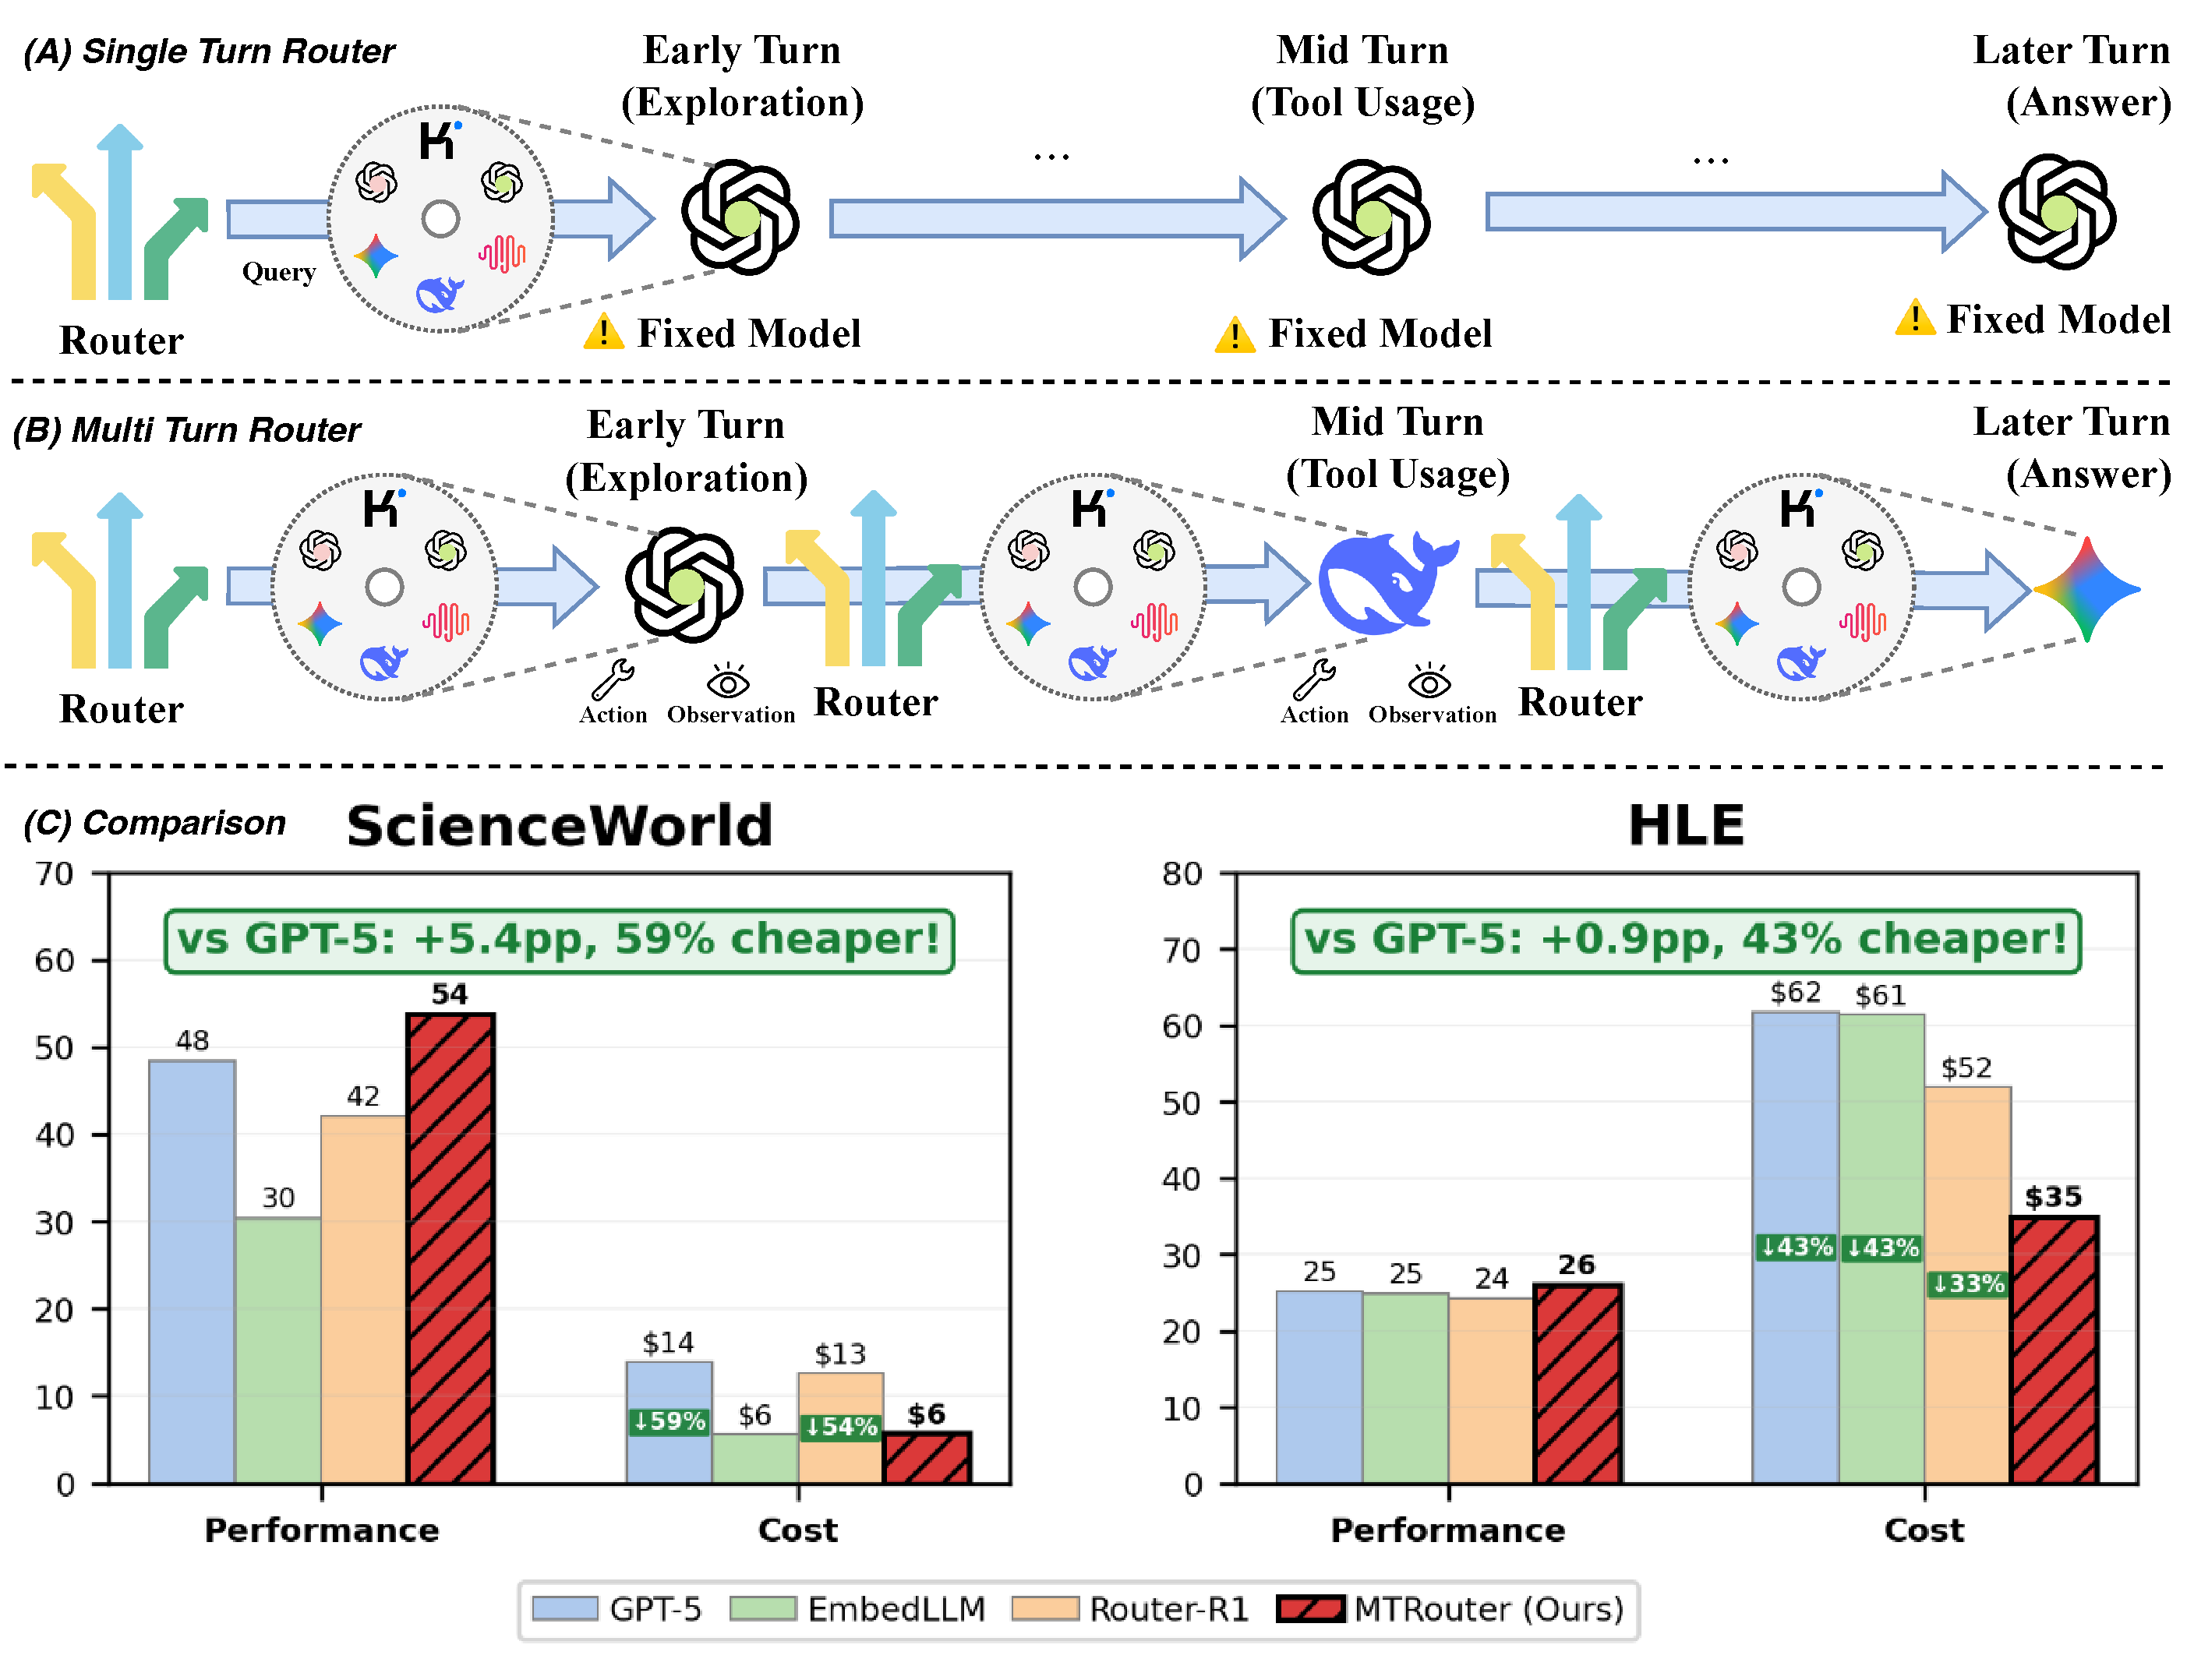
\includegraphics[width=\linewidth]{figures/toy-example.pdf}
\caption{\textbf{Top:} a single-turn (episode-level) router selects one model and keeps it fixed throughout the episode. \textbf{Middle:} a multi-turn router can adapt the model choice across turns based on the changing interaction state. \textbf{Bottom:} \method achieves a better performance--cost trade-off than representative baselines on ScienceWorld~\citep{wang2022scienceworld} and Humanity's Last Exam (HLE)~\citep{phan2025humanitysexam}.}
\label{fig:toy_example}
\vspace{-1.0em}
\end{figure}

This economic pressure is framed by a stark disparity in the current model landscape: frontier models provide state-of-the-art reasoning (like \texttt{claude-opus-4.5}\footnote{\url{https://www.anthropic.com/claude/opus}}, \texttt{gpt-5\footnote{\url{https://openai.com/index/gpt-5-system-card}}}) but are often two orders of magnitude more expensive than their lightweight counterparts (like \texttt{DeepSeek-v3.2~\citep{liu2025deepseek}, Kimi-K2~\citep{team2025kimi}}). To mitigate costs, prior work has explored single-turn (episode-level) routing, which selects a single model at the start of an episode based on the initial prompt (Figure~\ref{fig:toy_example}, Top). However, this static approach is inherently sub-optimal for long-horizon tasks. A single episode often consists of heterogeneous steps, ranging from high-stakes strategic planning to routine tool invocations and data formatting. Using a frontier model for every turn is wasteful, yet relying solely on a cheap model risks catastrophic failure during critical junctures.


This observation motivates multi-turn (turn-level) routing, where the agent adaptively switches between models at each step of the interaction (Figure~\ref{fig:toy_example}, Middle). While promising, multi-turn routing poses a significant predictive challenge: a router must assess whether a specific model choice at the current turn will jeopardize the final outcome dozens of steps later. Simple heuristics or localized error detection are often insufficient to capture the long-term impact of a model's performance on the entire trajectory.

We propose \textbf{\method}, which learns an \emph{outcome estimator} from logged trajectories.
The estimator maps a history--model pair to an estimate of the eventual episode outcome (terminal score/accuracy), using an error-aware adjustment to provide a stable training signal from offline data.
At inference time, the router selects the candidate model with the highest predicted outcome at each turn, and the episode is evaluated under fixed cost and turn limits.

Empirically, \method delivers consistent gains in both performance and cost.
On ScienceWorld (test), it improves average score from 48.4 (GPT-5) to 53.8 while reducing total cost by 58.7\%; on HLE (test), it reaches competitive accuracy while reducing total cost by 43.4\%.
It also generalizes under semantic distribution shift (OOD), maintaining improved outcomes with substantial cost savings (Table~\ref{tab:combined_results}).
Beyond aggregate metrics, our analysis shows that multi-turn routing is not ``switch more'': \method reaches success with fewer model switches than Router-R1~\cite{zhang2025router}, is more tolerant to transient errors, and exhibits structured model usage and emergent specialization across tools/actions (Figures~\ref{fig:cost_switches}--\ref{fig:action_by_model}).

Our key contributions are as follows:

\begin{itemize}[nolistsep, noitemsep, leftmargin=*]
\item We introduce \textbf{\method}, which learns an outcome estimator over history--model pairs from offline trajectories and performs turn-level routing in multi-turn agent episodes.
\item We evaluate on ScienceWorld and HLE (test and OOD) with a fixed candidate pool, and show consistent improvements in both performance and total cost over strong routing baselines, including Router-R1 and a representative commercial router.
\item We provide analyses that connect these gains to concrete routing behaviors, including fewer unnecessary switches, improved error recovery, and emergent specialization across tools/actions.
\end{itemize}